%\ifx\wholebook\relax\else
%\documentclass[twoside]{book}
%\usepackage[active]{srcltx}
%\usepackage[LY1]{fontenc}
%\usepackage{url}
\makeatletter
\def\url@leostyle{%
  \@ifundefined{selectfont}{\def\UrlFont{\sf}}{\def\UrlFont{\sffamily}}}
\makeatother
% Now actually use the newly defined style.
\urlstyle{leo}

\usepackage{graphicx}
\def\etc{{\textit{etc}}}
\def\eg{{\textit{e.g.}}}
\def\ie{{\textit{i.e.}}}
\def\cf{{\textit{c.f.}}\ }
\def\erf{\mathop{\textrm{erf}}}
\def\sign{\mathop{\textrm{sign}}}
\def\prob{\mathop{\textrm{Prob}}}
\def\var{\mathop{\textrm{var}}}
\def\mod{\mathop{\textrm{mod}}}
\def\cor{\mathop{\textrm{cor}}}
\def\cov{\mathop{\textrm{cov}}}
\def\cl{\mathop{\textrm{CL}}}
\def\kg{\mathop{\textrm{Kg}}}
\def\patstyle#1{{\textsc #1}}
\def\th{^{\mathop{\textrm{th}}}}
%\def\st#1{^{\mathop{\rm #1}}}
\def\note#1{\begin{quote}{\textbf{Note:}} #1\end{quote}}
\def\braket#1{\left\langle #1\right\rangle}
\def\order#1{\let\o=#1$\mathcal{O}$\ifx\o 1$\left(n\right)$\else$\left(n^{#1}\right)$\fi}
%\newtheorem{privListing}{Listing}[chapter]
%\newenvironment{listing}{\vskip 3ex\hrule\vskip 1ex\begin{privListing}}{\end{privListing}\hrule\vskip 1ex}
\newtheorem{privExample}{Code example}[chapter]
\newenvironment{codeExample}{\begin{privExample}\begin{quote}\tt}{\end{quote}\end{privExample}}
\def\relboxl#1#2{\hbox to #1\hsize{#2\hfil}}
\def\relboxc#1#2{\hbox to #1\hsize{\hfil #2\hfil}}
\def\relboxr#1#2{\hbox to #1\hsize{\hfil #2}}
\def\transpose#1{\textbf{#1}^{\mathop\textrm{T}}}
\def\inverse#1{\textbf{#1}^{-1}}
%\def\tm{$^{\mathop{\rm TM}}$}
\def\tm{ }
\newenvironment{mainEquation}{\marginpar[\vspace{3 ex} Main
equation$\Rightarrow$]{\vspace{3 ex}$\Leftarrow$Main
equation}\begin{equation}}{\end{equation}}
\def\rubrique#1{\paragraph{#1}\hfil\par\noindent}

%\begin{document}
%\fi

\chapter{Function evaluation}
\label{ch:function} \vspace{1 ex}
\begin{flushright}
{\textsl Qu'il n'y ait pas de r\'eponse n'excuse pas l'absence de
questions.}\footnote{The absence of answer does not justify the
absence of question.}\\ Claude Roy
\end{flushright}
\vspace{1 ex} Many mathematical functions used in numerical
computation are defined by an integral, by a recurrence formula or
by a series expansion. While such definitions can be useful to a
mathematician, they are usually quite complicated to implement on
a computer. For one, not every programmer knows how to evaluate an
integral numerically\footnote{The good news is that they will if
they read the present book (\cf chapter \ref{ch:integration}).}.
Then, there is the problem of accuracy. Finally, the evaluation of
the function as defined mathematically is often too slow to be
practical.

Before computers were heavily used, however, people had already
found efficient ways of evaluating complicated functions. These
methods are usually precise enough and extremely fast. This
chapter exposes several functions that are important for
statistical analysis. The Handbook of Mathematical Functions by
Abramovitz and Stegun \cite{AbrSteg} contains a wealth of such
function definitions and describes many ways of evaluating them
numerically. Most approximations used in this chapter have been
taken from this book.

This chapter opens on general considerations on how to implement
the concept of function. Then, polynomials are discussed as an
example of concrete function implementation. The rest of this
chapter introduces three classical functions: the error function,
the gamma function and the beta function. We shall use this
functions in chapters \ref{ch:statistics} and \ref{ch:estimation}.
Because these functions are fundamental functions used in many
areas of mathematics they are implemented as library functions ---
such as a sine, log or exponential --- instead of using the
general function formalism described in the first section.

Figure \ref{fig:functions} shows the diagram of the Smalltalk classes
described in this chapter.
\begin{figure}
\centering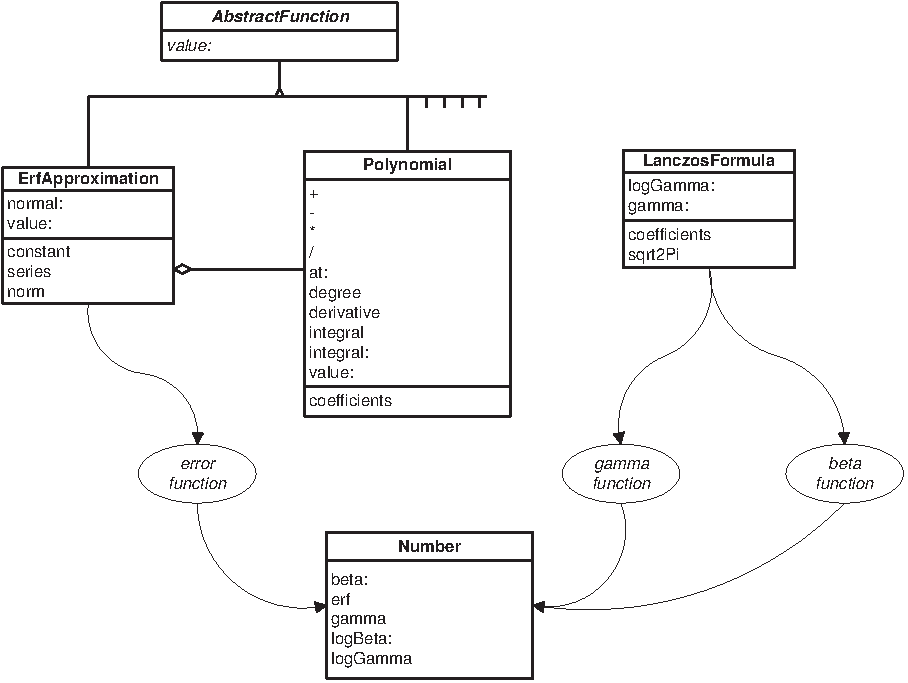
\includegraphics[width=10cm]{Figures/FunctionS}
\caption{Smalltalk classes related to functions}
\label{fig:functions}
\end{figure}
Here we have used special notations to indicate that the functions
are implemented as library functions. The functions are
represented by oval and arrows shows which class is used to
implement a function for the class {\texttt Number}.

\section{Function concept}
\label{sec:function}
A mathematical function is an object
associating a value to a variable. If the variable is a single
value one talks about a one variable function. If the variable is
an array of values one talks about a multi-variable function.
Other types of variables are possible but will not be covered in
this book.

We shall assume that the reader is familiar with elementary
concepts about functions, namely derivatives and integrals. We
shall concentrate mostly on implementation issues.

\section{Function -- Smalltalk implementation}
\label{sec:stFunction}
A mathematical function is an object
associating a value to a variable. If the variable is a single
value one talks about a one variable function. If the variable is
an array of values one talks about a multi-variable function.
Other types of variables are possible but will not be covered in
this book.

We shall assume that the reader is familiar with elementary
concepts about functions, namely derivatives and integrals. We
shall concentrate mostly on implementation issues.

\marginpar{Figure \ref{fig:functions} with
the box {\textbf AbstractFunction} grayed.} A function in Smalltalk
can be readily implemented with a block closure. Block closures in
Smalltalk are treated like objects; thus, they can be manipulated
as any other objects. For example the one variable function
defined as:
\begin{equation}
f\left( x \right)={1 \over x},
\end{equation}
can be implemented in Smalltalk as:
\begin{equation}
\hbox{\texttt f := [:x | 1 / x]}.
\end{equation}
Evaluation of a block closure is supplied by the method value:.
For example, to compute the inverse of 3, one writes:
\begin{equation}
\hbox{\texttt f value: 3}.
\end{equation}

If the function is more complex a block closure may not be the
best solution to implement a function. Instead a class can be
created with some instance variables to hold any constants and/or
partial results. In order to be able to use functions
indifferently implemented as block closures or as classes, one
uses polymorphism. Each class implementing a function must
implement a method value:. Thus, any object evaluating a function
can send the same message selector, namely value:, to the variable
holding the function.

To evaluate a multi-variable function, the argument of the method
value: is an Array or a vector (\cf section
\ref{sec:linearalgebra}). Thus, in Smalltalk multi-variable
functions can follow the same polymorphism as for one-variable
functions.

\section{Polynomials}
\label{sec:polynomial}
 Polynomials are quite important in
numerical methods because they are often used in approximating
functions. For example, section \ref{sec:errorFunction} shows how
the error function can be approximated with the product of normal
distribution times a polynomial.

Polynomials are also useful in approximating functions, which are
determined by experimental measurements in the absence of any
theory on the nature of the function. For example, the output of a
sensor detecting a coin is dependent on the temperature of the
coin mechanism. This temperature dependence cannot be predicted
theoretically because it is a difficult problem. Instead, one can
measure the sensor output at various controlled temperatures.
These measurements are used to determine the coefficients of a
polynomial reproducing the measured temperature variations. The
determination of the coefficients is performed using a polynomial
least-square fit (\cf section \ref{sec:lsfpol}). Using this
polynomial the correction for a given temperature can be evaluated
for any temperature within the measured range.

The reader is advised to read carefully the implementation section as many techniques are introduced at this occasion.
Later on those techniques will be mentioned with no further explanations.

\subsection{Mathematical definitions}
\label{sec:polymath} A polynomial is a special mathematical
function whose value is computed as follows:
\begin{equation}
\label{eq:polynomialDef}P\left(x\right)=\sum_{k=0}^{n}a_k x^k.
\end{equation}
$n$ is called the degree of the polynomial. For example, the
second order polynomial
\begin{equation}
\label{eq:polynomialExample} x^2 -3x + 2
\end{equation}
represents a parabola crossing the $x$-axis at points 1 and 2 and
having a minimum at $x= 2/3$. The value of the polynomial at the
minimum is $-1/4$.

In equation \ref{eq:polynomialDef} the numbers $a_0, \ldots a_n$
are called the coefficients of the polynomial. Thus, a polynomial
can be represented by the array $\left\{ a_0, \ldots a_n
\right\}$. For example, the polynomial of equation
\ref{eq:polynomialExample} is represented by the array $\left\{
2,-3,1 \right\}$.

Evaluating equation \ref{eq:polynomialDef} as such is highly
inefficient since one must raise the variable to an integral power
at each term. The required number of multiplication is of the
order of $n^2$. There is of course a better way to evaluate a
polynomial. It consists of factoring out $x$ before the evaluation
of each term\footnote{This is actually the first program I ever
wrote in my first computer programming class. Back in 1969, the
language in fashion was ALGOL.}. The following formula shows the
resulting expression:
\begin{mainEquation}
\label{eq:horner}
\left(x\right)=a_0+x\left\{a_1+x\left[a_2+x\left(a_3+\cdots\right)\right]\right\}
\end{mainEquation}
Evaluating the above expression now requires only multiplications.
The resulting algorithm is quite straightforward to implement.
Expression \ref{eq:horner} is called Horner's rule because it was
first published by W.G. Horner in 1819. 150 years earlier,
however, Isaac Newton was already using this method to evaluate
polynomials.

In section \ref{sec:newton} we shall requires the derivative of a
function. For polynomials this is rather straightforward. The
derivative is given by:
\begin{equation}
\label{eq:polynomialDeriv}{dP\left(x\right)\over
dx}=\sum_{k=1}^{n}k a_k x^{k-1}.
\end{equation}
Thus, the derivative of a polynomial with $n$ coefficients is
another polynomial, with $n-1$ coefficients\footnote{Notice the
change in the range of the summation index in equation
\ref{eq:polynomialDeriv}.} derived from the coefficients of the
original polynomial as follows:
\begin{equation}
a^\prime _k=\left(k+1\right)a_{k+1}\mbox{\quad for
$k=0,\ldots,n-1$}.
\end{equation}
For example, the derivative of \ref{eq:polynomialExample} is
$2x-3$.

The integral of a polynomial is given by:
\begin{equation}
\int_0^xP\left(t\right)dt=\sum_{k=0}^{n}{a_k \over k+1} x^{k+1}.
\end{equation}
Thus, the integral of a polynomial with $n$ coefficients is
another polynomial, with $n+1$  coefficients derived from the
coefficients of the original polynomial as follows:
\begin{equation}
\bar{a}_k={a_{k-1}\over k}\mbox{\quad for $k=1,\ldots,n+1$}.
\end{equation}
For the integral, the coefficient $\bar{a}_0$ is arbitrary and
represents the value of the integral at $x=0$. For example the
integral of \ref{eq:polynomialExample} which has the value -2 at
$x=0$ is the polynomial
\begin{equation}
{x^3\over 3}-{3 ^2\over2}+2x-2.
\end{equation}
Conventional arithmetic operations are also defined on polynomials
and have the same properties\footnote{The set of polynomials is a
vector space in addition to being a ring.} as for signed integers.

Adding or subtracting two polynomials yields a polynomial whose
degree is the maximum of the degrees of the two polynomials. The
coefficients of the new polynomial are simply the addition or
subtraction of the coefficients of same order.

Multiplying two polynomials yields a polynomial whose degree is
the product of the degrees of the two polynomials. If $\left\{
a_0,\ldots,a_n \right\}$ and $\left\{ b_0,\ldots,b_n \right\}$ are
the coefficients of two polynomials, the coefficients of the
product polynomial are given by:
\begin{equation}
\label{eq:polMult} c_k = \sum_{i+j=k}a_i b_j \mbox{\quad for
$k=0,\ldots,n+m$}.
\end{equation}
In equation \ref{eq:polMult} the coefficients $a_k$ are treated as
0 if $k>n$. Similarly the coefficients $n_k$ are treated as 0 if
$k>m$.

Dividing a polynomial by another is akin to integer division with
remainder. In other word the following equation:
\begin{equation}
P\left(x\right)=Q\left(x\right)\cdot
T\left(x\right)+R\left(x\right).
\end{equation}
uniquely defines the two polynomials $Q\left(x\right)$, the
quotient, and $R\left(x\right)$, the remainder, for any two given
polynomials $P\left(x\right)$ and $T\left(x\right)$. The algorithm
is similar to the algorithm taught in elementary school for
dividing integers \cite{Knuth2}.

\subsection{Polynomial --- Smalltalk implementation}
As we have seen a polynomial is uniquely defined by its
coefficients. Thus, the creation of a new polynomial instance must
have the coefficients given. Our implementation assumes that the
first element of the array containing the coefficients is the
coefficient of the constant term, the second element the
coefficient of the linear term ($x$), and so on.

The method {\texttt value} evaluates the polynomial at the supplied
argument. This methods implements equation \ref{eq:horner}.

The methods {\texttt derivative} and {\texttt integral} return each a new
instance of a polynomial. The method {\texttt integral:} must have an
argument specifying the value of the integral of the polynomial at
0. A convenience {\texttt integral} method without a<rgument is
equivalent to call the method {\texttt integral} with argument 0.

The implementation of polynomial arithmetic is rarely used in
numerical computation though. It is, however, a nice example to
illustrate a technique called double dispatching. Double
dispatching is described in appendix (\cf section
\ref{sec:doubledisp}). The need for double dispatching comes for
allowing an operation between object of different nature. In the
case of polynomials operations can be defined between two
polynomials or between a number and a polynomial. In short, double
dispatching allows one to identify the correct method based on the
type of the two arguments.

\marginpar{Figure \ref{fig:functions}
with the box {\textbf Polynomial} grayed.}
Being a special case of a function a polynomial must of course implement the behavior of
functions as discussed in section \ref{sec:stFunction}.
Here is a code example on how to use the class {\texttt PMPolynomial}.
\begin{listing}{Smalltalk}

| polynomial |
 polynomial := PMPolynomial coefficients: #(2 -3 1).
 polynomial value: 1.
\end{listing}
The code above creates an instance of the class {\texttt
PMPolynomial} by giving the coefficient of the polynomial. In
this example the polynomial $x^2-3x+2$. The final line of the code
computes the value of the polynomial at $x=1$.

The next example shows how to manipulate polynomials in symbolic
form.
\begin{listing}{Smalltalk}

 | pol1 pol2 polynomial polD polI |
 pol1:= PMPolynomial coefficients: #(2 -3 1).
 pol2:= PMPolynomial coefficients: #(-3 7 2 1).
 polynomial := pol1 * pol2.
 polD := polynomial derivative.
 polI := polynomial integral.
\end{listing}
The first line creates the  polynomial of example
\ref{eq:polynomialExample}. The second line creates the polynomial
$x^3+2x^2+7x-3$. The third line of the code creates a new
polynomial, product of the first two. The last two lines create
two polynomials, respectively the derivative and the integral of
the polynomial created in the third line.

Listing \ref{ls:polynomial} shows the Smalltalk implementation of
the class {\texttt PMPolynomial}.

A beginner may have been tempted to make {\texttt PMPolynomial} a
subclass of {\texttt Array} to spare the need for an instance
variable. This is of course quite wrong. An array is a subclass of
{\texttt Collection}. Most methods implemented or inherited by {\texttt
Array} have nothing to do with the behavior of a polynomial as a
mathematical entity.

Thus, a good choice is to make the class {\texttt PMPolynomial} a
subclass of Object. It has a single instance variable, an Array
containing the coefficients of the polynomial.

It is always a good idea to implement a method {\texttt printOn:} for
each class. This method is used by many system utilities to
display an object in readable form, in particular the debugger and
the inspectors. The standard method defined for all objects simply
displays the name of the class. Thus, it is hard to decide if two
different variables are pointing to the same object. Implementing
a method {\texttt printOn:} allows displaying parameters particular to
each instance so that the instances can easily be identified. It
may also be used in quick print on the {\texttt Transcript} and may
save you the use on an inspector while debugging. Implementing a
method {\texttt printOn:} for each class that you create is a good
general practice, which can make your life as a Smalltalker much
easier.

Working with indices in Smalltalk is somewhat awkward for
mathematical formulas because the code is quite verbose. In
addition a mathematician using Smalltalk for the first time may be
disconcerted with all indices starting at 1 instead of 0.
Smalltalk, however, has very powerful iteration methods, which
largely compensate for the odd index choice, odd for a
mathematician that is. In fact, an experienced Smalltalker seldom
uses indices explicitly as Smalltalk provides powerful iterator
methods.

The method {\texttt value:} uses the Smalltalk iteration method {\texttt
inject:into:} (\cf section \ref{sec:injectinto}). Using this
method requires storing the coefficients in reverse order because
the first element fed into the method {\texttt inject:into:}
corresponds to the coefficient of the largest power of $x$. It
would certainly be quite inefficient to reverse the order of the
coefficients at each evaluation. Since this requirement also
simplifies the computation of the coefficients of the derivative
and of the integral, reversing of the coefficients is done in the
creation method to make things transparent.

The methods {\texttt derivative} and {\texttt integral} return a new
instance of the class {\texttt PMPolynomial}. They do not modify the
object receiving the message. This is also true for all operations
between polynomials. The methods {\texttt derivative} and {\texttt
integral} use the method {\texttt collect:} returning a collection of
the values returned by the supplied block closure at each argument
(\cf section \ref{sec:collect}).

The method {\texttt at:} allows one to retrieve a given coefficient.
To ease readability of the multiplication and division methods,
the method {\texttt at:} has been defined to allow for indices
starting at 0. In addition this method returns zero for any index
larger than the polynomial's degree. This allows being lax with
the index range. In particular, equation \ref{eq:polMult} can be
coded exactly as it is.

The arithmetic operations between polynomials are implemented
using double dispatching. This is a general technique widely used
in Smalltalk (and all other languages with dynamical typing)
consisting of selecting the proper method based on the type of the
supplied arguments. Double dispatching is explained in section
\ref{sec:doubledisp}.

\note{Because Smalltalk is a dynamically typed language, our
implementation of polynomial is also valid for polynomials with
complex coefficients.}

\begin{listing}[label=lst:polynomial]{Smalltalk}
{Smalltalk implementation of the polynomial class}
$$\halign{ #\hfil&\quad#\hfil\cr {\sl Class}& {\Large\bf PMPolynomial}\cr
{\sl Subclass of }&{\tt Object}\cr\noalign{\vskip 1ex}

{\sl Instance variable names:}&\parbox[t]{4 in}{\tt  coefficients }\cr\noalign{\vskip 1ex}}$$


Class methods
{\parskip 1ex\par\noindent}
{\bf coefficients:} {\tt anArray}
\begin{verbatim}
    ^self new initialize: anArray reverse
\end{verbatim}



Instance methods
{\parskip 1ex\par\noindent}
{\bf *} {\tt aNumberOrPolynomial}
\begin{verbatim}
    ^aNumberOrPolynomial timesPolynomial: self
\end{verbatim}
{\bf +} {\tt aNumberOrPolynomial}
\begin{verbatim}
    ^aNumberOrPolynomial addPolynomial: self
\end{verbatim}
{\bf -} {\tt aNumberOrPolynomial}
\begin{verbatim}
    ^aNumberOrPolynomial subtractToPolynomial: self
\end{verbatim}
{\bf /} {\tt aNumberOrPolynomial}
\begin{verbatim}
    ^aNumberOrPolynomial dividingPolynomial: self
\end{verbatim}
{\bf addNumber:} {\tt aNumber}
\begin{verbatim}
    | newCoefficients |
    newCoefficients := coefficients reverse.
    newCoefficients at: 1 put: newCoefficients first + aNumber.
    ^self class new: newCoefficients
\end{verbatim}
{\bf addPolynomial:} {\tt aPolynomial}
\begin{verbatim}
    ^self class new: ( ( 0 to: (self degree max: aPolynomial degree)) 
                collect: [ :n | ( aPolynomial at: n) + ( self at: n) ])
\end{verbatim}
{\bf at:} {\tt anInteger}
\begin{verbatim}
    ^anInteger < coefficients size
        ifTrue: [ coefficients at: ( coefficients size - anInteger) ]
        ifFalse: [ 0 ]
\end{verbatim}
{\bf coefficients}
\begin{verbatim}
    ^coefficients deepCopy
\end{verbatim}
{\bf degree}
\begin{verbatim}
    ^coefficients size - 1
\end{verbatim}
{\bf derivative}
\begin{verbatim}
    | n |
    n := coefficients size.
    ^self class new: ( ( coefficients 
    					collect: [ :each | n := n - 1. each * n]) reverse copyFrom: 2 to: coefficients size)
\end{verbatim}
{\bf dividingPolynomial:} {\tt aPolynomial}
\begin{verbatim}
    ^ (self dividingPolynomialWithRemainder: aPolynomial) first
\end{verbatim}
{\bf dividingPolynomialWithRemainder:} {\tt aPolynomial}
\begin{verbatim}
    | remainderCoefficients quotientCoefficients n m norm 
                                                      quotientDegree |
    n := self degree.
    m := aPolynomial degree.
    quotientDegree := m - n.
    quotientDegree < 0
        ifTrue: [ ^Array with: ( self class new: #(0)) with: 
                                                         aPolynomial].
    quotientCoefficients := Array new: quotientDegree + 1.
    remainderCoefficients := ( 0 to: m) collect: [ :k | aPolynomial 
                                                               at: k].
    norm := 1 / coefficients first.
    quotientDegree to: 0 by: -1
        do: [ :k | | x |
              x := ( remainderCoefficients at: n + k + 1) * norm.
              quotientCoefficients at: (quotientDegree + 1 - k) put: 
                                                                    x.
              (n + k - 1) to: k by: -1
                do: [ :j | 
                remainderCoefficients at: j + 1 put: 
                            ( ( remainderCoefficients at: j + 1) - ( 
                                                x * (self at: j - k)))
                ].
            ].
    ^ Array with: ( self class new: quotientCoefficients reverse)
           with: ( self class new: ( remainderCoefficients copyFrom: 1 to: n))
\end{verbatim}
{\bf initialize:} {\tt anArray}
\begin{verbatim}
    coefficients := anArray.
    ^ self
\end{verbatim}
{\bf integral}
\begin{verbatim}
    ^ self integral: 0
\end{verbatim}
{\bf integral:} {\tt aValue}
\begin{verbatim}
    | n |
    n := coefficients size + 1.
    ^ self class new: ( ( coefficients collect: [ :each | n := n - 1. 
                                  each / n]) copyWith: aValue) reverse
\end{verbatim}
{\bf printOn:} {\tt aStream}
\begin{verbatim}
    | n firstNonZeroCoefficientPrinted |
    n := 0.
    firstNonZeroCoefficientPrinted := false.
    coefficients reverse do:
        [ :each |
          each = 0
            ifFalse:[ firstNonZeroCoefficientPrinted
                            ifTrue: [ aStream space.
                                         each < 0
                                            ifFalse:[ aStream 
                                                         nextPut: $+].
                                         aStream space.
                                        ]
                            ifFalse:[ firstNonZeroCoefficientPrinted 
                                                             := true].
                          ( each = 1 and: [ n > 0])
                            ifFalse:[ each printOn: aStream].
                          n > 0
                            ifTrue: [ aStream nextPutAll: ' X'.
                                         n > 1
                                            ifTrue: [ aStream 
                                                          nextPut: $^.
                                                         n printOn: 
                                                              aStream.
                                                        ].
                                        ].
                        ].
         n := n + 1.
        ].
\end{verbatim}
{\bf subtractToPolynomial:} {\tt aPolynomial}
\begin{verbatim}
    ^self class new: ( ( 0 to: (self degree max: aPolynomial degree)) 
                collect: [ :n | ( aPolynomial at: n) - ( self at: n)])
\end{verbatim}
{\bf timesNumber:} {\tt aNumber}
\begin{verbatim}
    ^self class new: ( coefficients reverse collect: [ :each | each * aNumber])
\end{verbatim}
{\bf timesPolynomial:} {\tt aPolynomial}
\begin{verbatim}
    | productCoefficients degree|
    degree := aPolynomial degree + self degree.
    productCoefficients := (degree to: 0 by: -1)
            collect:[ :n | | sum |
                      sum := 0.
                      0 to: (degree - n)
                        do: [ :k | sum := (self at: k) * (aPolynomial 
                                        at: (degree - n - k)) + sum].
                      sum
                    ].
    ^self class new: productCoefficients
\end{verbatim}
{\bf value:} {\tt aNumber}
\begin{verbatim}
    ^coefficients inject: 0 into: [ :sum :each | sum * aNumber + each]
\end{verbatim}


\end{listing}

Listing \ref{ls:polynomialNumber} shows the listing of the methods
used by the class Number as part of the double dispatching of the
arithmetic operations on polynomials.

\begin{listing}[label=lst:polynomialNumber]{Smalltalk}
{Method of class {\texttt Number} related to polynomials}
$$\halign{ #\hfil&\quad#\hfil\cr {\sl Class}& {\Large\bf Number}\cr
{\sl Subclass of }&{\tt Magnitude}\cr\noalign{\vskip 1ex}
}$$


Instance methods
{\parskip 1ex\par\noindent}
{\bf addPolynomial:} {\tt aPolynomial}
\begin{verbatim}
    ^aPolynomial addNumber: self
\end{verbatim}
{\bf dividingPolynomial:} {\tt aPolynomial}
\begin{verbatim}
    ^aPolynomial timesNumber: (1 / self)
\end{verbatim}
{\bf subtractToPolynomial:} {\tt aPolynomial}
\begin{verbatim}
    ^aPolynomial addNumber: self negated
\end{verbatim}
{\bf timesPolynomial:} {\tt aPolynomial}
\begin{verbatim}
    ^aPolynomial timesNumber: self
\end{verbatim}


\end{listing}

\section{Error function}
\label{sec:errorFunction}
\begin{figure}
\centering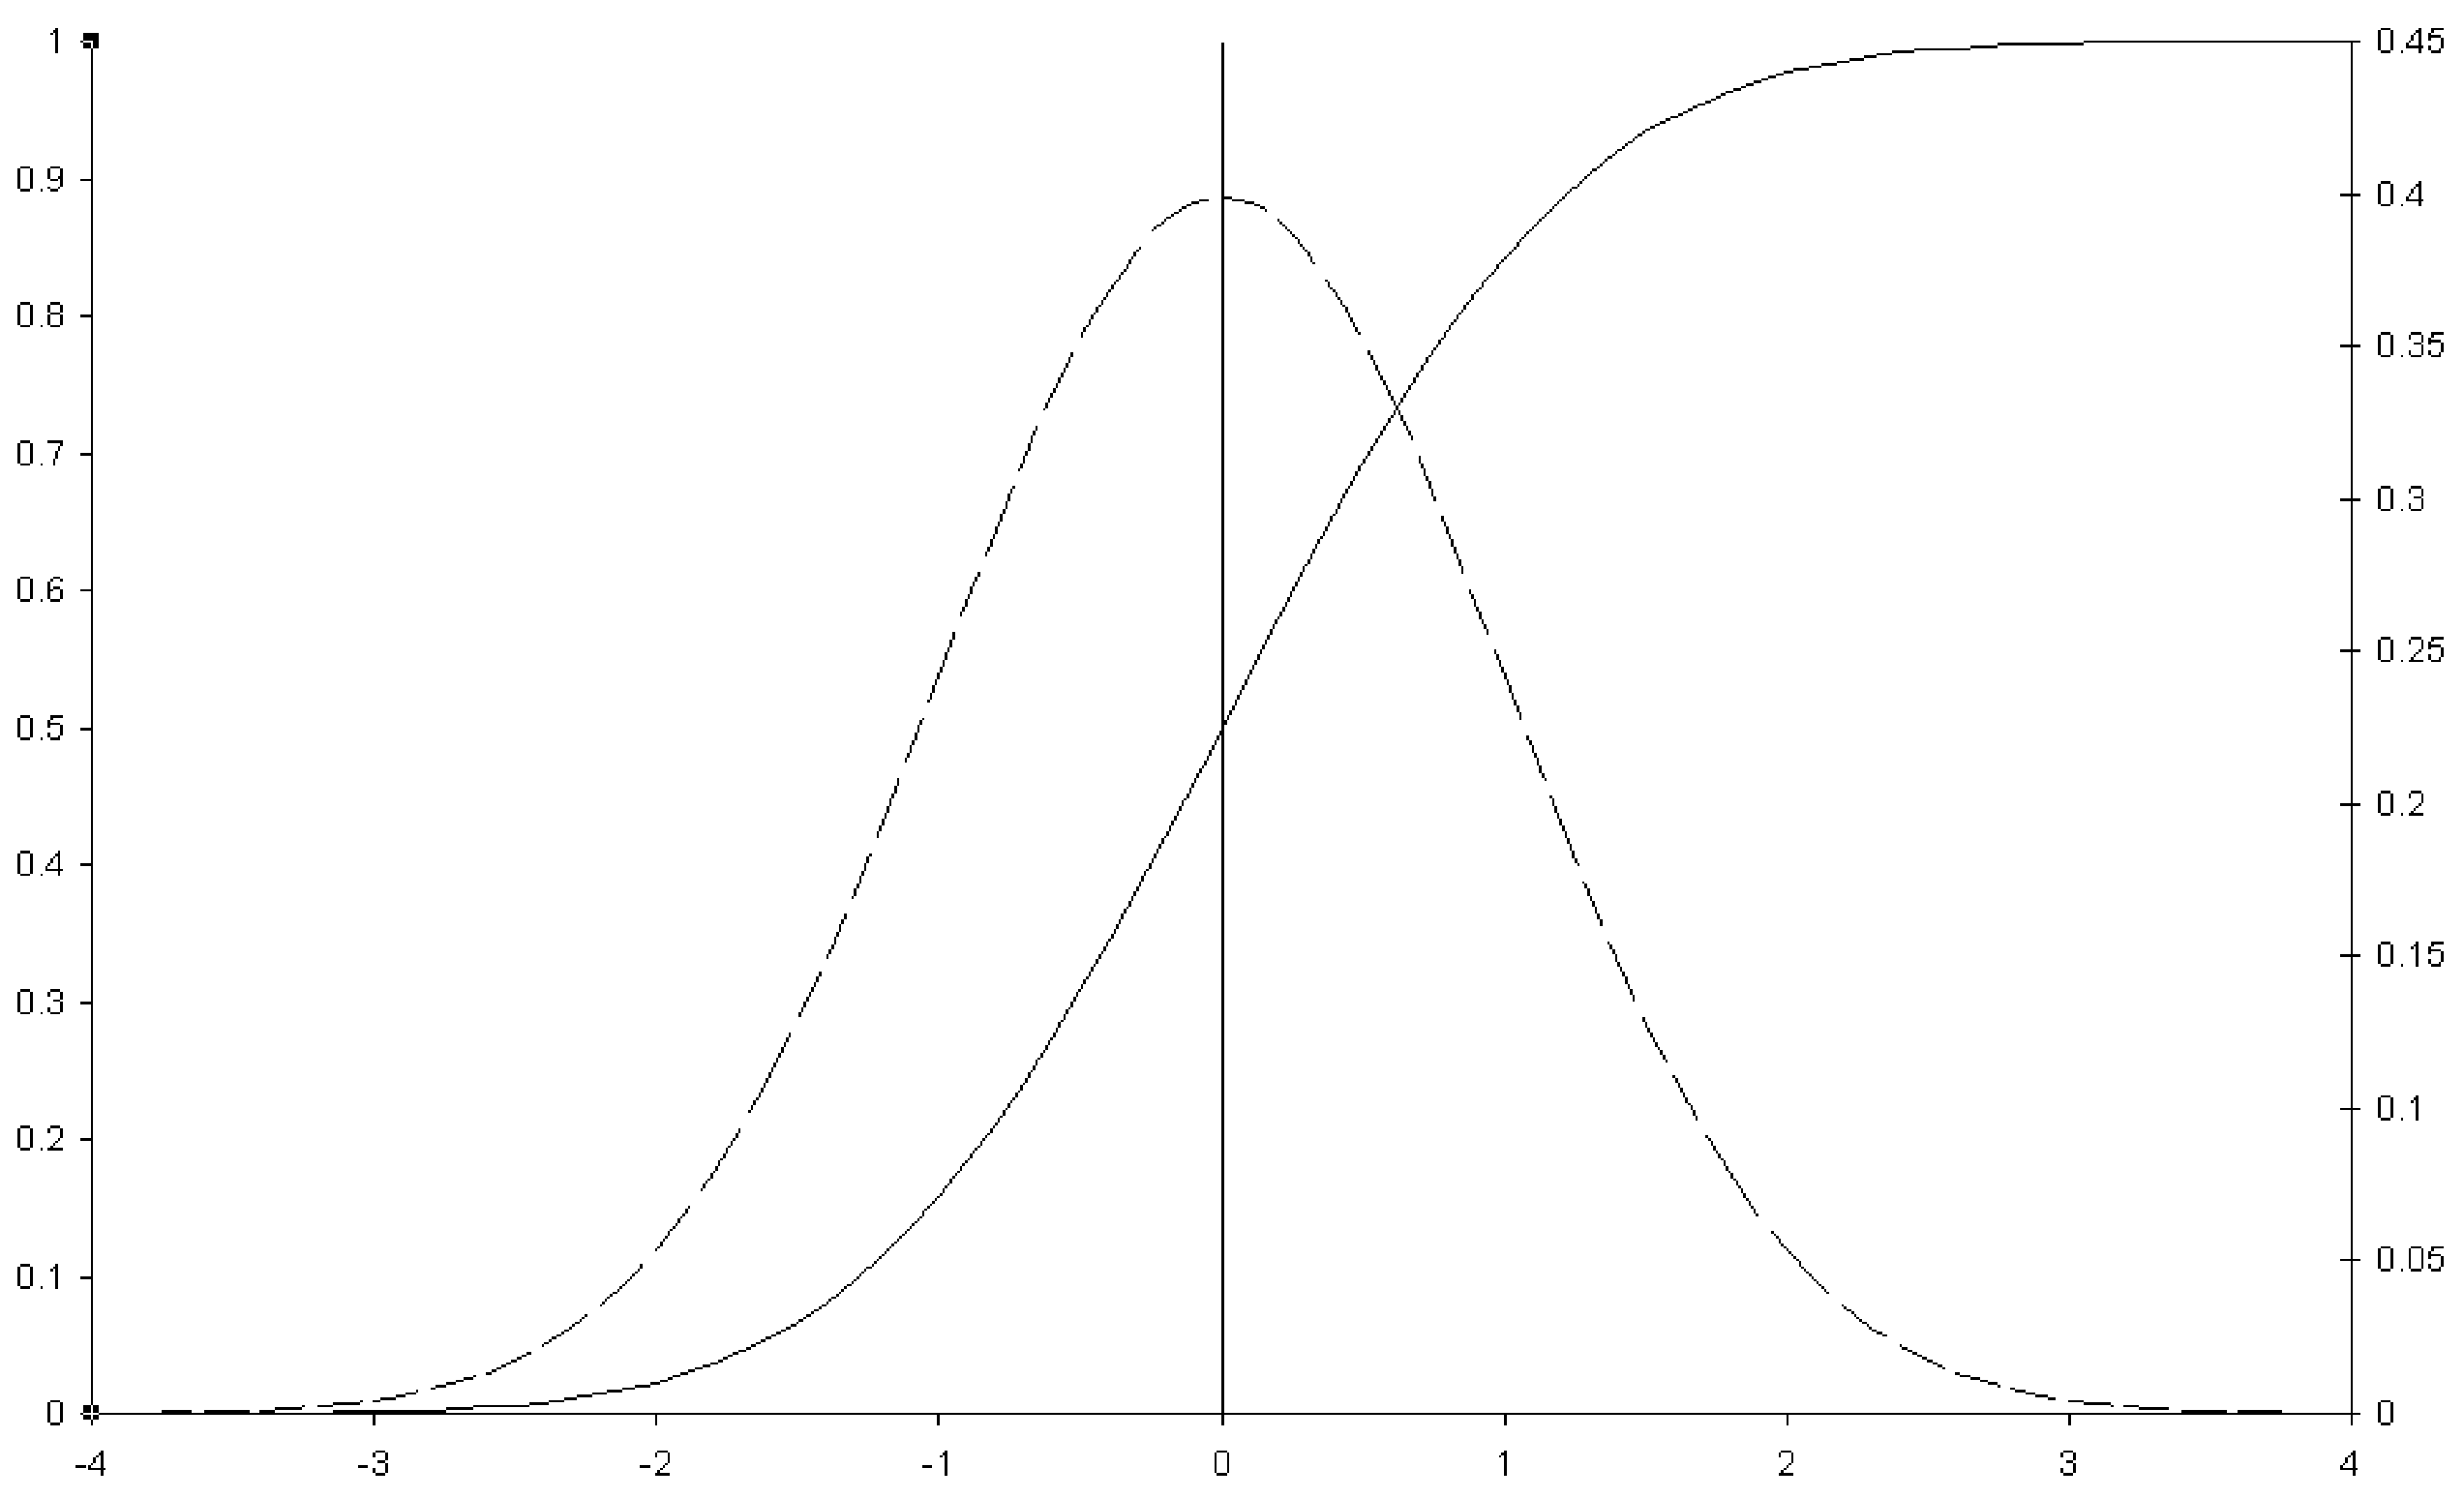
\includegraphics[width=8cm]{Figures/ErrorFunction}
\caption{The error function and the normal
distribution}\label{fig:errorFunction}
\end{figure}
The error function is the integral of the normal distribution. The
error function is used in statistics to evaluate the probability
of finding a measurement larger than a given value when the
measurements are distributed according to a normal distribution.
Figure \ref{sec:errorFunction} shows the familiar bell-shaped
curve of the probability density function of the normal
distribution (dotted line) together with the error function (solid
line).

In medical sciences one calls {\textsl centile} the value of the error
function expressed in percent. For example, obstetricians look
whether the weight at birth of the first born child is located
below the $10^{\mbox{th}}$ centile or above the $90^{\mbox{th}}$
centile to assess a risk factor for a second
pregnancy\footnote{\cf footnote \ref{ft:steer} on page
\pageref{ft:steer}}.

\subsection{Mathematical definitions}
\label{sec:errorFunctionDef} Because it is the integral of the
normal distribution, the error function, $\erf\left(x\right)$,
gives the probability of finding a value lower than $x$ when the
values are distributed according to a normal distribution with
mean 0 and standard deviation 1. The mean and the standard
deviation are explained in section \ref{sec:moments}. This
probability is expressed by the following integral\footnote{In
\cite{AbrSteg} and \cite{Press}, the error function is defined as:
$$\erf\left(x\right)={2 \over \sqrt{\pi}}\int_0^x e^{-{t^2 \over 2
}}dt$$.}:
\begin{equation}
\erf\left(x\right)={1 \over \sqrt{2\pi}}\int_{-\infty}^x e^{-{t^2
\over 2 }}dt
\end{equation}
The result of the error function lies between 0 and 1.

One could carry out the integral numerically, but there exists
several good approximations. The following formula is taken from
\cite{AbrSteg}.
\begin{mainEquation}
\label{eq:erf} \erf\left(x\right)={1 \over \sqrt{2\pi}}e^{-{x^2
\over 2 }}\sum_{i=1}^5 a_i r\left(x\right)^i\mbox{\quad for $x\ge
0$}.
\end{mainEquation}
where
\begin{equation}
\label{eq:erfpol}r\left(x\right)={1 \over {1-0.2316419x}}.
\end{equation}
and
\begin{equation}
\label{eq:erfconst}\left\{ \begin{array}{lr}a_1 =&0.31938153 \\
a_2 =&-0.356563782
\\a_3 =&1.7814779372 \\ a_4 =&-1.821255978 \\ a_5 =&1.330274429
\end{array}\right.
\end{equation}
The error on this formula is better than $7.5\times10^{-8}$ for
negitive $x$. To compute the value for positive values, one uses
the fact that:
\begin{mainEquation}
\label{eq:erfneg} \erf\left(x\right)=1-\erf\left(-x\right).
\end{mainEquation}
When dealing with a general Gaussian distribution with average
$\mu$ and standard deviation $\sigma$ it is convenient to define a
generalized error function as:
\begin{equation}
\erf\left(x;\mu,\sigma\right)={1 \over
\sqrt{2\pi\sigma^2}}\int_{-\infty}^x e^{-{{\left(x-\mu\right)}^2
\over 2 \sigma^2}}dt.
\end{equation}
A simple change of variable in the integral shows that the
generalized error function can be obtained from the error function
as:
\begin{mainEquation}
\erf\left(x;\mu,\sigma\right)=\erf\left({x-\mu\over\sigma}\right).
\end{mainEquation}
Thus, one can compute the probability of finding a measurement $x$
within the interval $\left[\mu - t \cdot \sigma,\mu + t \cdot
\sigma\right] $ when the measurements are distributed according to
a Gaussian distribution with average $\mu$ and standard deviation
$\sigma$:
\begin{equation}
\label{eq:normaccept}
\prob\left({\left|x-\mu\right|\over\sigma}\le t\right)=2 \cdot
\erf\left(t\right)-1.\mbox{\quad for $t\ge 0$}.
\end{equation}

\rubrique{Example}
\def\w{2.85}\def\av{3.39}\def\st{0.44}
 Now we can give the answer to the problem of deciding
whether a pregnant woman needs special attention during her second
pregnancy. Let the weight at birth of her first child be $\w\kg$.
and let the duration of her first pregnancy be 39 weeks. In this
case measurements over a representative sample of all births
yielding healthy babies have an average of $\av\kg$ and a standard
deviation of $\st\kg$\footnote{\label{ft:steer}This is the
practice at the department of obstetrics and gynecology of the
Chelsea $\&$ Westminster Hospital of London. The numbers are
reproduced with permission of Prof. P.J. Steer.}. The probability
of having a weight of birth smaller than that of the woman's first
child is:
\begin{eqnarray*}
\prob\left(\mathop{\textrm Weight}\le \w\kg \right) & = &
\erf\left({\w-\av\over\st}\right),\\ & = & 11.2\%.
\end{eqnarray*}
According to current practice, this second pregnancy does not
require special attention.

\subsection{Error function --- Smalltalk implementation}
\label{sec:sterrorfunction} \marginpar{Figure \ref{fig:functions}
with the box {\texbf ErfApproximation} grayed.} The error function is
implemented as a single method for the class Number. Thus,
computing the centile of our preceding example is simply coded as:
\begin{codeExample}
\begin{verbatim}

 | weight average stDev centile |
 weight := 2.85.
 average := 3.39.
 stDev := 0.44.
 centile := ( ( weight - average) / stDev) erf * 100.
\end{verbatim}
\end{codeExample}
If you want to compute the probability for a measurement to lay
within 3 standard deviations from its mean, you need to evaluate
the following expression using equation \ref{eq:normaccept}:
\begin{codeExample}
\begin{verbatim}

 3 errorFunction * 2 - 1
\end{verbatim}
\end{codeExample}
If one needs to use the error function as a function, one must use
it inside a block closure. In this case one defines a function
object as follows:
\begin{codeExample}
\begin{verbatim}

| errorFunction |
errorFunction := [ :x | x errorFunction ].
\end{verbatim}
\end{codeExample}
Listing \ref{ls:errorFunction} shows the Smalltalk implementation
of the error function.

In Smalltalk we are allowed to extend existing classes. Thus, the
public method to evaluate the error function is implemented as a
method of the base class {\texttt Number}. This method uses the class,
{\texttt DhbErfApproximation}, used to store the constants of equation
\ref{eq:erfconst} and evaluate the formula of equations
\ref{eq:erf} and \ref{eq:erfpol}. In our case, there is no need to
create a separate instance of the class {\texttt DhbErfApproximation}
at each time since all instances would actually be exactly
identical. Thus, the class {\texttt DhbErfApproximation} is a
singleton class. A singleton class is a class, which can only
create a single instance \cite{GoF}. Once the first instance is
created, it is kept in a class instance variable. Any subsequent
attempt to create an additional instance will return a pointer to
the class instance variable holding the first created instance.

One could have implemented all of these methods as class methods
to avoid the singleton class. In Smalltalk, however, one tends to
reserve class method for behavior needed by the structural
definition of the class. So, the use of a singleton class is
preferable. A more detailed discussion of this topic can be found
in \cite{StDesPat}.

\begin{listing}
Smalltalk implementation of the Error function
\label{ls:errorFunction}
$$\halign{ #\hfil&\quad#\hfil\cr {\sl Class}& {\Large\bf Number}\cr
{\sl Subclass of }&{\tt Magnitude}\cr\noalign{\vskip 1ex}
}$$


Instance methods
{\parskip 1ex\par\noindent}
{\bf errorFunction}
\begin{verbatim}
    ^DhbErfApproximation new value: self

\end{verbatim}


$$\halign{ #\hfil&\quad#\hfil\cr {\sl Class}& {\Large\bf DhbErfApproximation}\cr
{\sl Subclass of }&{\tt Object}\cr\noalign{\vskip 1ex}

{\sl Instance variable names:}&\parbox[t]{4 in}{\tt  constant series norm }\cr\noalign{\vskip 1ex}
{\sl Class variable names:}&\parbox[t]{4 in}{\tt  UniqueInstance }\cr\noalign{\vskip 1ex}}$$


Class methods
{\parskip 1ex\par\noindent}
{\bf new}
\begin{verbatim}
    UniqueInstance isNil
        ifTrue: [ UniqueInstance := super new initialize ].
    ^UniqueInstance
\end{verbatim}



Instance methods
{\parskip 1ex\par\noindent}
{\bf initialize}
\begin{verbatim}
    constant := 0.2316419.
    norm := 1 / ( Float pi * 2) sqrt.
    series := DhbPolynomial coefficients: #( 0.31938153 -0.356563782 
                               1.781477937 -1.821255978 1.330274429). 
\end{verbatim}
{\bf normal:} {\tt aNumber}
\begin{verbatim}
    ^[ ( aNumber squared * -0.5) exp * norm]
            when: ExAll do: [ :signal | signal exitWith: 0]
\end{verbatim}
{\bf value:} {\tt aNumber}
\begin{verbatim}
    | t |
    aNumber = 0
        ifTrue: [ ^0.5].
    aNumber > 0
        ifTrue: [ ^1- ( self value: aNumber negated)].
    aNumber < -20
        ifTrue: [ ^0].
    t := 1 / (1 - (constant * aNumber)).
    ^( series value: t) * t * (self normal: aNumber)
\end{verbatim}


\end{listing}

\section{Gamma function}
The gamma function is used in many mathematical functions. In this
book, the gamma function is needed to compute the normalization
factor of several probability density functions (\cf sections
\ref{sec:gammadist} and \ref{sec:chitest}). It is also needed to
compute the beta function (\cf section \ref{sec:betafunc}).

\subsection{Mathematical definitions}
\label{sec:gammafunc} The Gamma function is defined by the
following integral, called Euler's integral\footnote{Leonard Euler
to be precise as the Euler family produced many mathematicians.}:
\begin{equation}
\label{eq:gammafunc} \Gamma\left(x\right)=\int_0^\infty t^x
e^{-t}dt
\end{equation}
From equation \ref{eq:gammafunc} a recurrence formula can be
derived:
\begin{equation}
\label{eq:gammarec} \Gamma\left(x+1\right)=x \cdot
\Gamma\left(x\right)
\end{equation}
The value of the Gamma function can be computed for special values
of $x$:
\begin{equation}
\label{eq:gammaval}\left\{
\begin{array}{lr}\Gamma\left(1\right)=1\\\Gamma\left(2\right)=1
\end{array}\right.
\end{equation}
From \ref{eq:gammarec} and \ref{eq:gammaval}, the well-known
relation between the value of the Gamma function for positive
integers and the factorial can be derived:
\begin{equation}
\label{eq:gammafact} \Gamma\left(n\right)=\left(n-1\right)!
\mbox{\quad for $n>0$}.
\end{equation}
The most precise approximation for the Gamma function is given by
a formula discovered by Lanczos \cite{Press}:
\begin{mainEquation}
\label{eq:lanczos} \Gamma\left(x\right)\approx e^{\left(x+{5\over
2}\right)}\left(x+{5\over 2}\right){\sqrt{2\pi}\over x
}\left(c_0+\sum_{n=1}^6{c_n \over x + n}+\epsilon\right)
\end{mainEquation}
where
\begin{equation}
\label{eq:lanczosconst}\left\{ \begin{array}{lrl}c_0
=&1.000000000190015
\\c_1 =&76.18009172947146 \\ c_2 =&-86.50532032941677
\\c_3 =&24.01409824083091 \\ c_4 =&-1.231739572450155
\\ c_5 =&1.208650973866179&\cdot 10^{-3} \\ c_6 =&-5.395239384953&\cdot 10^{-6}
\end{array}\right.
\end{equation}
This formula approximates $\Gamma\left(x\right)$ for $x>1$ with
$\epsilon<2\cdot 10^{-10}$ . Actually, this remarkable formula can
be used to compute the gamma function of any complex number $z$
with $\Re\left(z\right)>1$ to the quoted precision. Combining
Lanczos' formula with the recurrence formula \ref{eq:gammarec} is
sufficient to compute values of the Gamma function for all
positive numbers.

For example, $\Gamma\left({3\over 2}\right)={\sqrt{\pi}\over 2}=
0.886226925452758$ whereas Lanczos formula yields the value
$0.886226925452754$, that is, an absolute error of $4\cdot
10^{-15} $. The corresponding relative precision is almost equal
to the floating-point precision of the machine on which this
computation was made.

Although this is seldom used, the value of the Gamma function for
negative non-integer numbers can be computed using the reflection
formula hereafter:
\begin{equation}
\label{eq:gammaneg} \Gamma\left(x\right)={\pi\over
\Gamma\left(1-x\right) \sin\pi x}
\end{equation}

In summary, the algorithm to compute the Gamma function for any
argument goes as follows:
\begin{enumerate}
  \textitem If $x$ is a non-positive integer ($x\le0$), raise an exception.
  \textitem If $x$ is smaller than or equal to 1 ($x<1$), use the recurrence formula \ref{eq:gammarec}.
  \textitem If $x$ is negative ($x<0$, but non integer), use the reflection
formula \ref{eq:gammaneg}.
  \textitem Otherwise use Lanczos' formula \ref{eq:lanczos}.
\end{enumerate}

One can see from the leading term of Lanczos' formula that the
gamma function raises faster than an exponential. Thus, evaluating
the gamma function for numbers larger than a few hundreds will
exceed the capacity of the floating number representation on most
machines. For example, the maximum exponent of a double precision
IEEE floating-point number is 1024. Evaluating directly the
following expression:
\begin{equation}
\label{eq:gammaovfl}
  {\Gamma\left(460.5\right)\over\Gamma\left(456.3\right)}
\end{equation}
will fail since $\Gamma\left(460.5\right)$ is larger than
$10^{1024}$. Thus, its evaluation yields a floating-point overflow
exception. It is therefore recommended to use the logarithm of the
gamma function whenever it is used in quotients involving large
numbers. The expression of equation \ref{eq:gammaovfl} is then
evaluated as:
\begin{equation}
  \exp\left[\ln\Gamma\left(460.5\right)-\ln\Gamma\left(456.3\right)\right]
\end{equation}
which yield the result $1.497\cdot 10^{11}$. That result fits
comfortably within the floating-point representation.

For similar reasons the leading factors of Lanczos formula are
evaluated using logarithms in both implementations.

\subsection{Gamma function --- Smalltalk implementation}
\marginpar{Figure \ref{fig:functions} with the box {\texbf
LanczosFormula} grayed.} Like the error function, the gamma
function is implemented as a single method of the class {\texttt
Number}. Thus, computing the gamma function of 2.5 is simply coded
as:
\begin{codeExample}
\begin{verbatim}

 2.5 gamma
\end{verbatim}
\end{codeExample}
To obtain the logarithm of the gamma function, you need to
evaluate the following expression:
\begin{codeExample}
\begin{verbatim}

 2.5 logGamma
\end{verbatim}
\end{codeExample}
Listing 11 shows the Smalltalk implementation of the gamma
function.

Here, the gamma function is implemented with two methods: one for
the class {\texttt Integer} and one for the class {\texttt Float}.
Otherwise, the scheme to define the gamma function is similar to
that of the error function. Please refer to section
\ref{sec:sterrorfunction} for detailed explanations.

Since the method factorial is already defined for integers in the
base classes, the gamma function has been defined using equation
\ref{eq:gammafact} for integers. An error is generated if one
attempts to compute the gamma function for non-positive integers.
The class {\texttt Number} delegates the computation of Lanczos'
formula to a singleton class. This is used by the non-integer
subclasses of {\texttt Number}: {\texttt Float} and {\texttt Fraction}.

The execution time to compute the gamma function for floating
argument given in Table \ref{tb:speed} in section \ref{sec:speed}.
\begin{listing}
Smalltalk implementation of the gamma function
\label{ls:gammafunc}
$$\halign{ #\hfil&\quad#\hfil\cr {\sl Class}& {\Large\bf Integer}\cr
{\sl Subclass of }&{\tt Number}\cr\noalign{\vskip 1ex}
}$$


Instance methods
{\parskip 1ex\par\noindent}
{\bf gamma}
\begin{verbatim}
    self > 0
        ifFalse: [ ^self error: 'Attempt to compute the Gamma 
        function of a non-positive integer'].
    ^( self - 1) factorial
\end{verbatim}


$$\halign{ #\hfil&\quad#\hfil\cr {\sl Class}& {\Large\bf Number}\cr
{\sl Subclass of }&{\tt Magnitude}\cr\noalign{\vskip 1ex}
}$$


Instance methods
{\parskip 1ex\par\noindent}
{\bf gamma}
\begin{verbatim}
    ^self > 1
        ifTrue: [ ^DhbLanczosFormula new gamma: self]
        ifFalse:[ self < 0
                     ifTrue: [ Float pi / ( ( Float pi * self) sin * ( 1 - self) gamma)]
                     ifFalse:[ ( DhbLanczosFormula new gamma: (self + 1)) / self]
                    ]
\end{verbatim}
{\bf logGamma}
\begin{verbatim}
    ^self > 1
        ifTrue: [ DhbLanczosFormula new logGamma: self]
        ifFalse: [ self > 0
                      ifTrue: [ ( DhbLanczosFormula new logGamma: (self + 1)) - self ln ]
                      ifFalse: [ ^self error: 'Argument for the log gamma function
                         must be positive']
                    ]
\end{verbatim}


$$\halign{ #\hfil&\quad#\hfil\cr {\sl Class}& {\Large\bf DhbLanczosFormula}\cr
{\sl Subclass of }&{\tt Object}\cr\noalign{\vskip 1ex}

{\sl Instance variable names:}&\parbox[t]{4 in}{\tt  coefficients sqrt2Pi }\cr\noalign{\vskip 1ex}
{\sl Class variable names:}&\parbox[t]{4 in}{\tt  UniqueInstance }\cr\noalign{\vskip 1ex}}$$


Class methods
{\parskip 1ex\par\noindent}
{\bf new}
\begin{verbatim}
    UniqueInstance isNil
        ifTrue: [ UniqueInstance := super new initialize ].
    ^ UniqueInstance
\end{verbatim}

Instance methods
{\parskip 1ex\par\noindent}
{\bf gamma:} {\tt aNumber}
\begin{verbatim}
    ^ (self leadingFactor: aNumber) exp * (self series: aNumber) 
        * sqrt2Pi / aNumber
\end{verbatim}
{\bf initialize}
\begin{verbatim}
    sqrt2Pi := ( Float pi * 2) sqrt.
    coefficients := #( 76.18009172947146 -86.50532032941677 
           24.01409824083091 -1.231739572450155 0.1208650973866179e-2 
           -0.5395239384953e-5).
    ^ self
\end{verbatim}
{\bf leadingFactor:} {\tt aNumber}
\begin{verbatim}
    | temp |
    temp := aNumber + 5.5.
    ^ (temp ln * ( aNumber + 0.5) - temp)
\end{verbatim}
{\bf logGamma:} {\tt aNumber}
\begin{verbatim}
    ^ (self leadingFactor: aNumber) + ((self series: aNumber) 
    * sqrt2Pi / aNumber) ln
\end{verbatim}
{\bf series:} {\tt aNumber}
\begin{verbatim}
    | term |
    term := aNumber.
    ^coefficients inject: 1.000000000190015
                        into: [ :sum :each | term := term + 1. each / term + sum ]
\end{verbatim}


\end{listing}

\section{Beta function}
\label{sec:betafunc} The beta function is directly related to the
gamma function. In this book, the beta function is needed to
compute the normalization factor of several probability density
functions (\cf sections \ref{sec:Ftest}, \ref{sec:ttest} and
\ref{sec:betadist}).
\subsection{Mathematical definitions}
The beta function is defined by the following integral:
\begin{equation}
\label{eq:betaint} B\left(x,y\right)=\int_0^1
t^{x-1}\left(1-t\right)^{y-1}dt
\end{equation}
The beta function is related to the gamma function with the
following relation:
\begin{equation}
B\left(x,y\right)={\Gamma\left(x\right)\Gamma\left(y\right)\over\Gamma\left(x+y\right)}
\end{equation}
Thus, computation of the beta function is directly obtained from
the gamma function. As evaluating the gamma function might
overflow the floating-point exponent (\cf discussion at the end of
section \ref{sec:gammafunc}), it is best to evaluate the above
formula using the logarithm of the gamma function.

\subsection{Beta function --- Smalltalk implementation}
\marginpar{Figure \ref{fig:functions} with the box {\texbf
LanczosFormula} grayed.} Like the error and gamma functions, the
gamma function is implemented as a single method of the class {\texttt
Number}. Thus, computing the beta function of 2.5 and 5.5 is
simply coded as:
\begin{codeExample}
\begin{verbatim}

2.5 beta: 5.5
\end{verbatim}
\end{codeExample} Computing the logarithm of the beta function of
2.5 and 5.5 is simply coded as:
\begin{codeExample}
\begin{verbatim}

2.5 logBeta: 5.5
\end{verbatim}
\end{codeExample}
Listing \ref{ls:betafunc} shows the
implementation of the beta function in Smalltalk.

\begin{listing}
Smalltalk implementation of the beta function
\label{ls:betafunc}
$$\halign{ #\hfil&\quad#\hfil\cr {\sl Class}& {\Large\bf Number}\cr
{\sl Subclass of }&{\tt Magnitude}\cr\noalign{\vskip 1ex}
}$$


Instance methods
{\parskip 1ex\par\noindent}
{\bf beta:} {\tt aNumber}
\begin{verbatim}
    ^ (self logBeta: aNumber) exp
\end{verbatim}
{\bf logBeta:} {\tt aNumber}
\begin{verbatim}
    ^ self logGamma + aNumber logGamma - ( self + aNumber) logGamma
\end{verbatim}


\end{listing}

%\ifx\wholebook\relax\else\end{document}\fi
